\documentclass[border=4pt]{standalone}
\usepackage{tikz}
\usetikzlibrary{positioning, arrows.meta, calc, fit, backgrounds}
\usepackage{amssymb}

\begin{document}
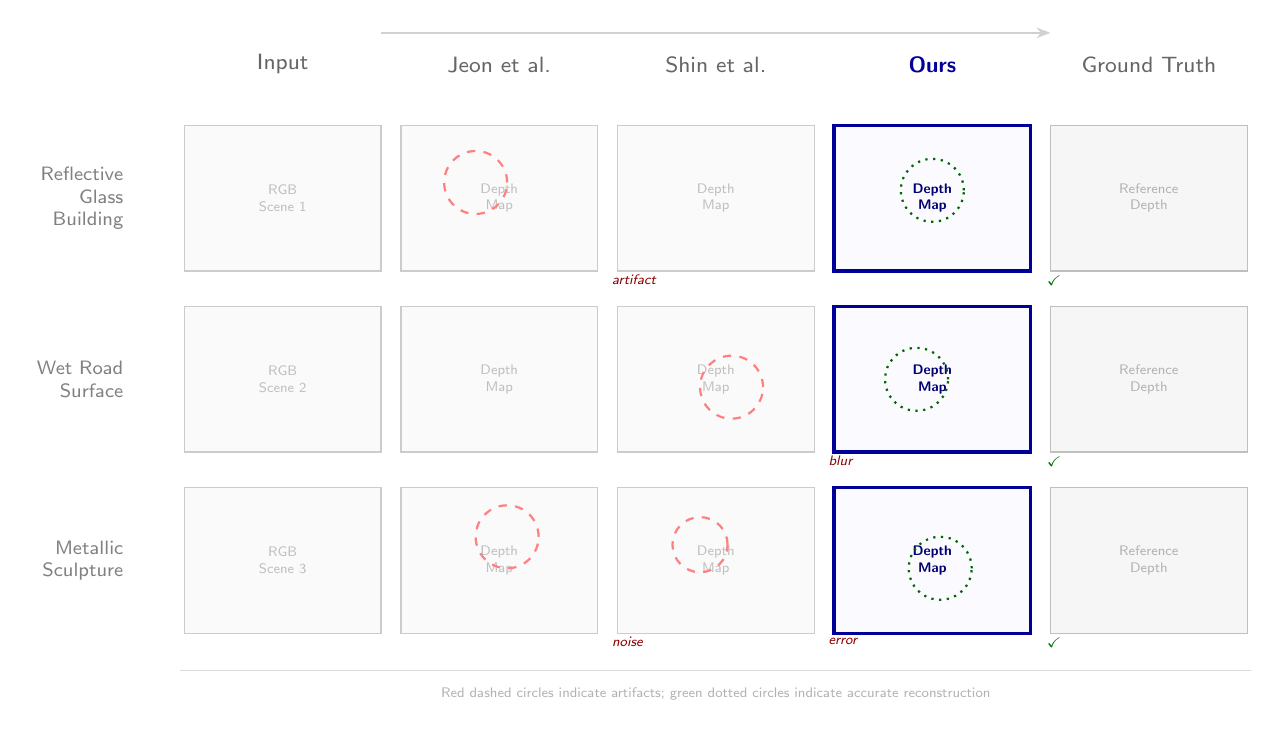
\begin{tikzpicture}[
    imgbox/.style={
        draw=gray!40, minimum width=2.5cm, minimum height=1.85cm,
        fill=gray!4, inner sep=0pt, align=center,
        font=\sffamily\tiny, text=black!25, line width=0.5pt
    },
    oursbox/.style={
        draw=blue!60!black, minimum width=2.5cm, minimum height=1.85cm,
        fill=blue!2, inner sep=0pt, align=center,
        font=\sffamily\tiny\bfseries, text=blue!45!black, line width=1.2pt
    },
    gtbox/.style={
        draw=gray!50, minimum width=2.5cm, minimum height=1.85cm,
        fill=gray!7, inner sep=0pt, align=center,
        font=\sffamily\tiny, text=black!30, line width=0.5pt
    },
    hdr/.style={font=\sffamily\footnotesize, text=black!60, align=center},
    slbl/.style={font=\sffamily\scriptsize, text=black!50, align=right},
    errcirc/.style={red!50, thick, dashed},
    goodcirc/.style={green!40!black, thick, dotted},
]

% Column x-coordinates
\def\cI{1.8}
\def\cA{4.55}
\def\cB{7.3}
\def\cO{10.05}
\def\cG{12.8}

% Row y-coordinates
\def\rI{-1.0}
\def\rII{-3.3}
\def\rIII{-5.6}

\def\hy{0.7}
\def\sx{-0.1}

% ====== HEADER ROW ======
\node[hdr] at (\cI, \hy) {Input};
\node[hdr] at (\cA, \hy) {Jeon et al.};
\node[hdr] at (\cB, \hy) {Shin et al.};
\node[hdr, font=\sffamily\footnotesize\bfseries, text=blue!60!black] at (\cO, \hy) {Ours};
\node[hdr] at (\cG, \hy) {Ground Truth};

% Flow arrow
\draw[-{Stealth[length=5pt]}, thick, black!18]
    ($({\cI+1.25}, \hy) + (0,0.4)$) -- ($({\cG-1.25}, \hy) + (0,0.4)$);

% ====== ROW 1: Reflective Glass Building ======
\node[slbl, anchor=east] at (\sx, \rI) {Reflective\\Glass\\Building};

\node[imgbox] (r1i) at (\cI, \rI) {RGB\\Scene~1};
\node[imgbox] (r1a) at (\cA, \rI) {Depth\\Map};
\node[imgbox] (r1b) at (\cB, \rI) {Depth\\Map};
\node[oursbox] (r1o) at (\cO, \rI) {Depth\\Map};
\node[gtbox] (r1g) at (\cG, \rI) {Reference\\Depth};

% Annotations Row 1
\draw[errcirc] ($(r1a.center) + (-0.3,0.2)$) circle (0.4cm);
\node[font=\sffamily\tiny\itshape, text=red!55!black, anchor=west] at ($(r1a.south east)+(0.05,-0.1)$) {artifact};
\draw[goodcirc] ($(r1o.center) + (0.0,0.1)$) circle (0.4cm);
\node[font=\sffamily\tiny\itshape, text=green!45!black, anchor=west] at ($(r1o.south east)+(0.05,-0.1)$) {\checkmark};

% ====== ROW 2: Wet Road Surface ======
\node[slbl, anchor=east] at (\sx, \rII) {Wet Road\\Surface};

\node[imgbox] (r2i) at (\cI, \rII) {RGB\\Scene~2};
\node[imgbox] (r2a) at (\cA, \rII) {Depth\\Map};
\node[imgbox] (r2b) at (\cB, \rII) {Depth\\Map};
\node[oursbox] (r2o) at (\cO, \rII) {Depth\\Map};
\node[gtbox] (r2g) at (\cG, \rII) {Reference\\Depth};

% Annotations Row 2
\draw[errcirc] ($(r2b.center) + (0.2,-0.1)$) circle (0.4cm);
\node[font=\sffamily\tiny\itshape, text=red!55!black, anchor=west] at ($(r2b.south east)+(0.05,-0.1)$) {blur};
\draw[goodcirc] ($(r2o.center) + (-0.2,0.0)$) circle (0.4cm);
\node[font=\sffamily\tiny\itshape, text=green!45!black, anchor=west] at ($(r2o.south east)+(0.05,-0.1)$) {\checkmark};

% ====== ROW 3: Metallic Sculpture ======
\node[slbl, anchor=east] at (\sx, \rIII) {Metallic\\Sculpture};

\node[imgbox] (r3i) at (\cI, \rIII) {RGB\\Scene~3};
\node[imgbox] (r3a) at (\cA, \rIII) {Depth\\Map};
\node[imgbox] (r3b) at (\cB, \rIII) {Depth\\Map};
\node[oursbox] (r3o) at (\cO, \rIII) {Depth\\Map};
\node[gtbox] (r3g) at (\cG, \rIII) {Reference\\Depth};

% Annotations Row 3
\draw[errcirc] ($(r3a.center) + (0.1,0.3)$) circle (0.4cm);
\node[font=\sffamily\tiny\itshape, text=red!55!black, anchor=west] at ($(r3a.south east)+(0.05,-0.1)$) {noise};
\draw[errcirc] ($(r3b.center) + (-0.2,0.2)$) circle (0.35cm);
\node[font=\sffamily\tiny\itshape, text=red!55!black, anchor=west] at ($(r3b.south east)+(0.05,-0.1)$) {error};
\draw[goodcirc] ($(r3o.center) + (0.1,-0.1)$) circle (0.4cm);
\node[font=\sffamily\tiny\itshape, text=green!45!black, anchor=west] at ($(r3o.south east)+(0.05,-0.1)$) {\checkmark};

% ====== BOTTOM NOTE ======
\draw[black!15, thin] (\cI-1.3, -7.0) -- (\cG+1.3, -7.0);
\node[font=\sffamily\tiny, text=black!30] at (7.3, -7.3)
    {Red dashed circles indicate artifacts; green dotted circles indicate accurate reconstruction};

\end{tikzpicture}
\end{document}